\section{Metodologia Proposta}
\label{sec:metodologia}

Nesta se\c{c}\~{a}o s\~{a}o detalhados o conjunto de dados cl\'{i}nico, o pipeline de pr\'{e}-processamento e aumento de dados, al\'{e}m da formula\c{c}\~{a}o matem\'{a}tica integral da arquitetura \textbf{RAPUNet-Zeta}.

\subsection{Base de Dados (Kvasir-SEG)}
A valida\c{c}\~{a}o experimental foi realizada sobre o \textit{Kvasir-SEG Dataset} \cite{kvasirseg}, um referencial aberto curado por m\'{e}dicos gastrenterologistas noruegueses do Hospital Universit\'{a}rio de Oslo. A base compreende 1.000 quadros de colonoscopia de alta resolu\c{c}\~{a}o, acompanhados por m\'{a}scaras bin\'{a}rias anotadas manualmente por especialistas, delimitando rigorosamente a regi\~{o}es de tecido displ\'{a}sico e neopl\'{a}sico. A Figura \ref{fig:dataset_samples} ilustra tr\^{e}s amostras t\'{i}picas do dataset com suas respectivas m\'{a}scaras de anota\c{c}\~{a}o cl\'{i}nica (\textit{Ground Truth}).

\begin{figure}[htbp]
    \centering
    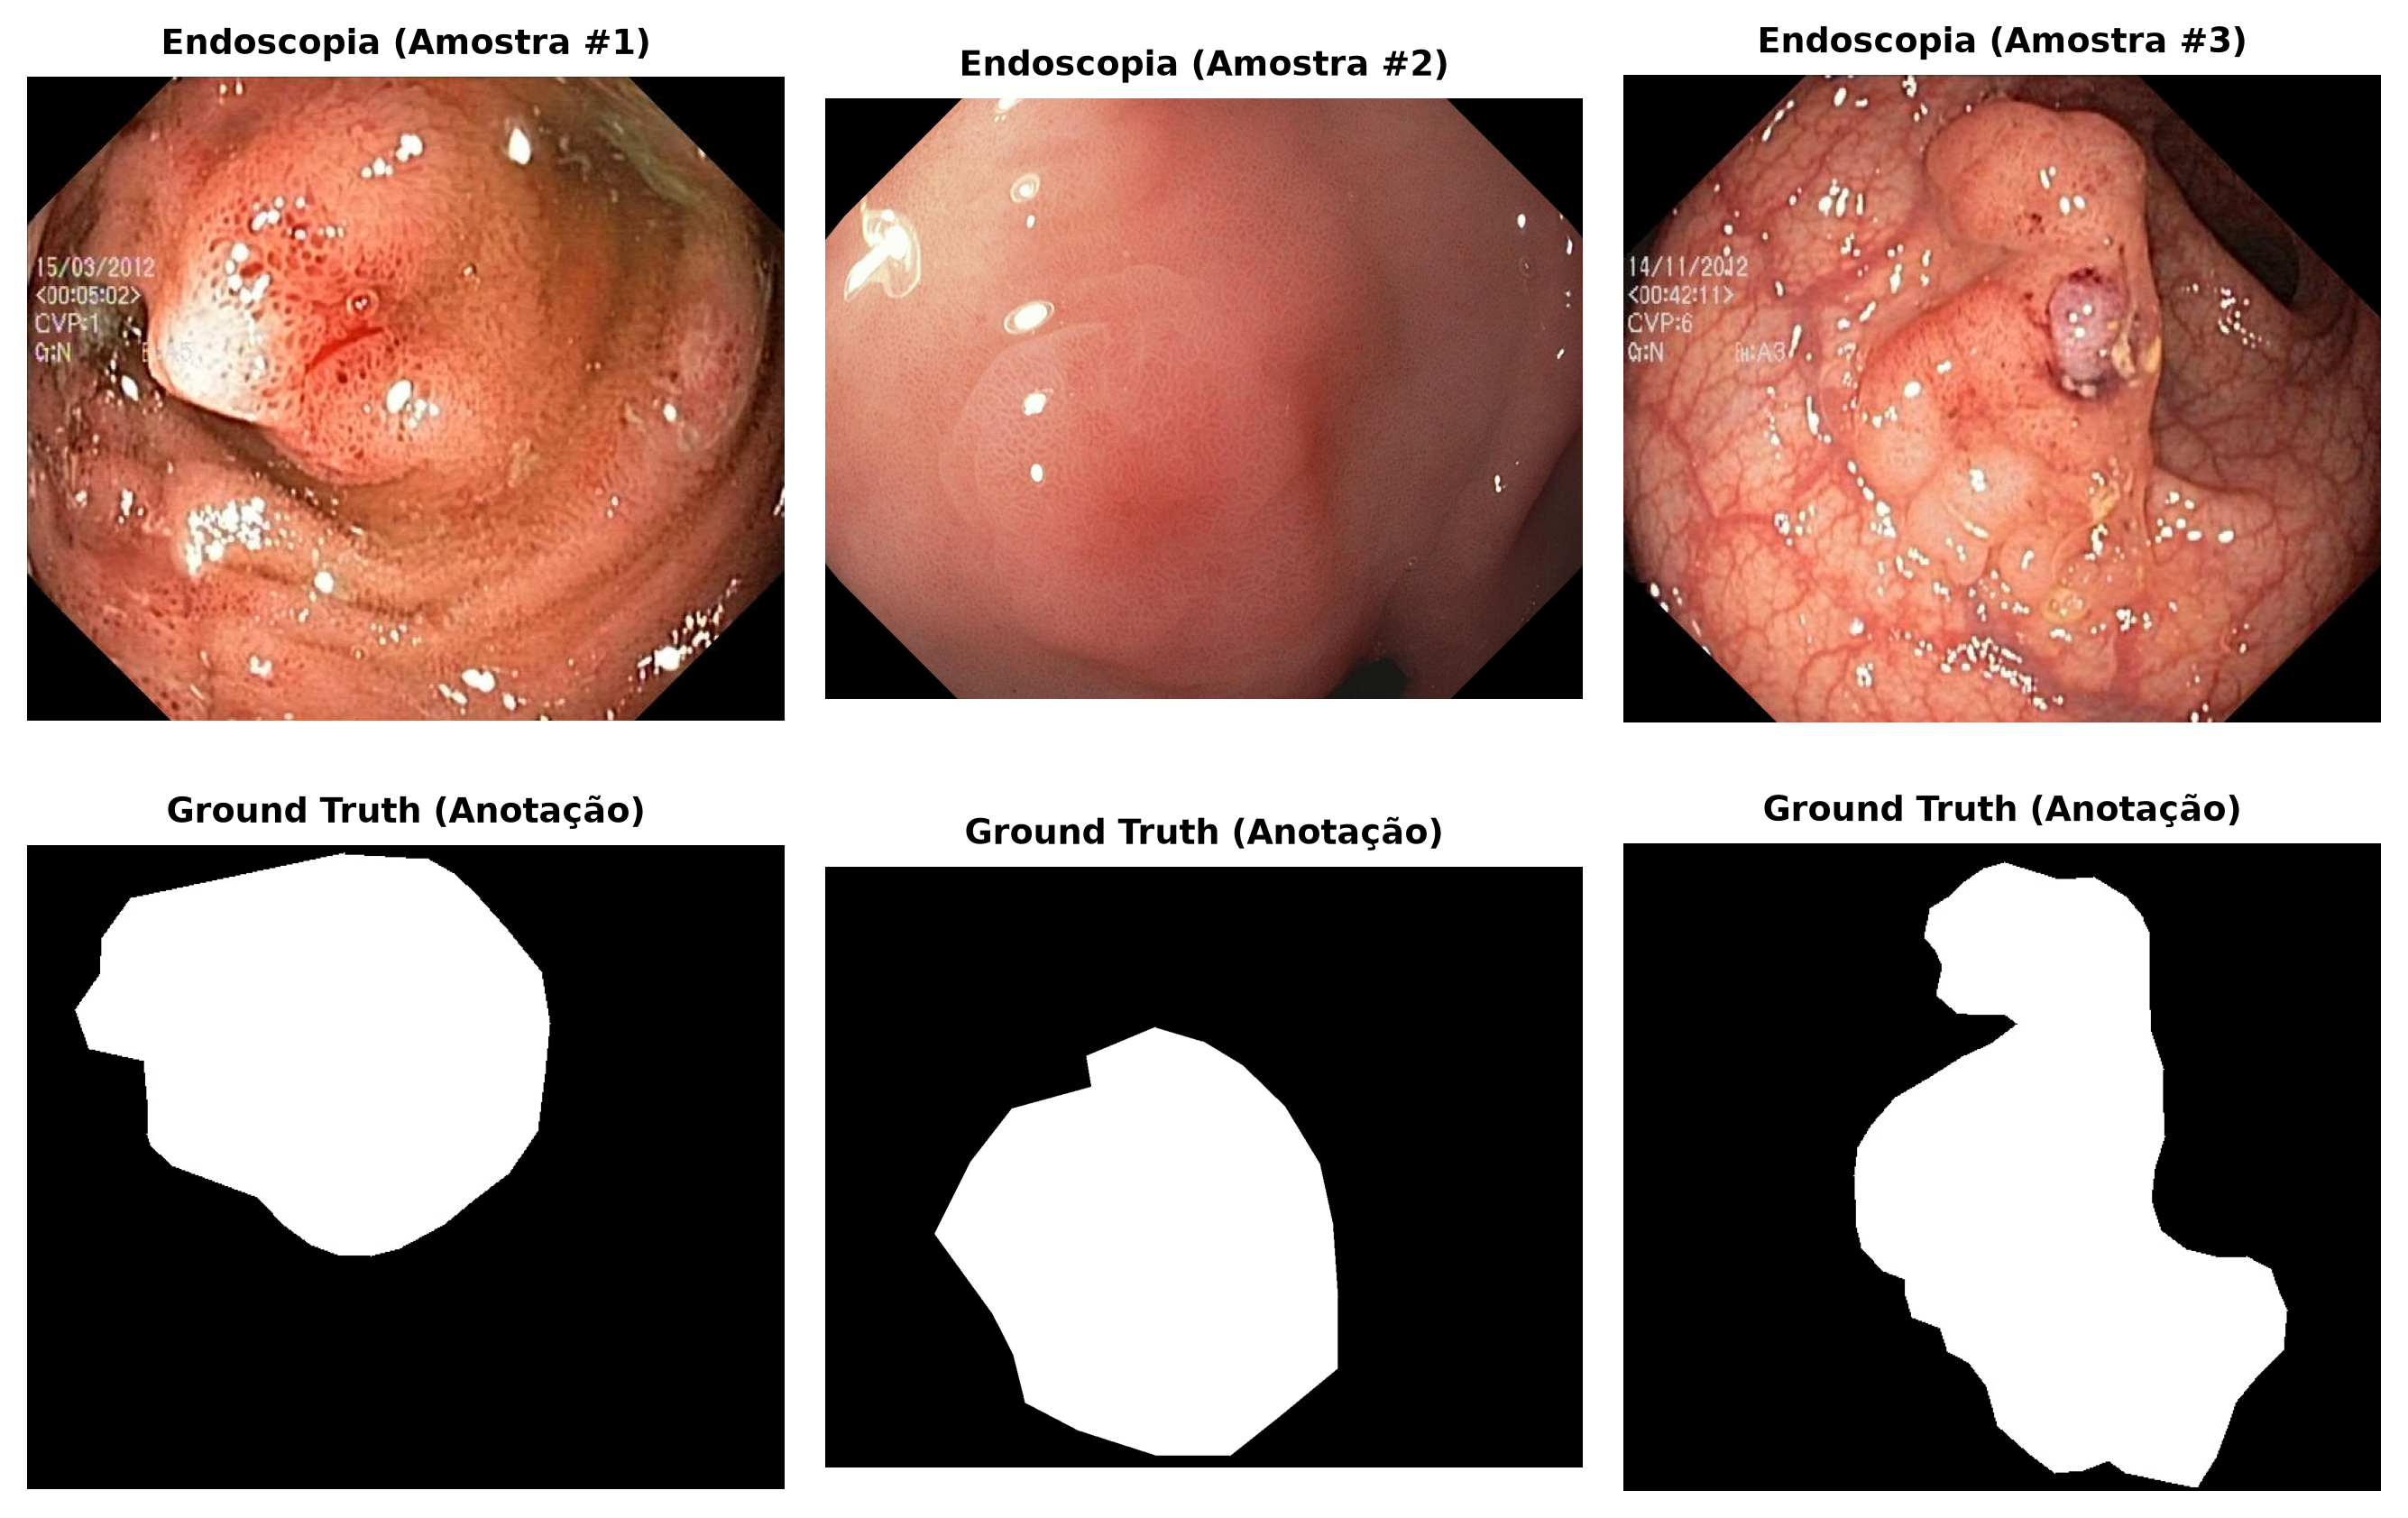
\includegraphics[width=0.88\textwidth]{figures/dataset_samples.png}
    \caption{Amostras representativas do dataset Kvasir-SEG \cite{kvasirseg}. Linha superior: imagens endosc\'{o}picas reais exibindo varia\c{c}\~{o}es morfol\'{o}gicas, luz especular e reflexos mucosos. Linha inferior: m\'{a}scaras bin\'{a}rias correspondentes geradas por m\'{e}dicos especialistas.}
    \label{fig:dataset_samples}
\end{figure}

Para adequa\c{c}\~{a}o \{a} mem\'{o}ria de v\'{i}deo (VRAM) e padroniza\c{c}\~{a}o da entrada do grafo computacional, todas as imagens e m\'{a}scaras foram redimensionadas para a resolu\c{c}\~{a}o can\^{o}nica de $352 \times 352$ pixels. As intensidades de pixel foram normalizadas para o intervalo cont\'{i}nuo $[0, 1]$. O particionamento dos dados utilizou 85\% das inst\^{a}ncias para o conjunto de treinamento e 15\% estritamente isoladas para teste e valida\c{c}\~{a}o cega.

\subsection{Pipeline de Aumento de Dados (Data Augmentation)}
Para mitigar o sobreajuste (\textit{overfitting}) decorrente do n\'{u}mero de par\^{a}metros do codificador profundo, estruturou-se uma esteira de aumento estoc\'{a}stico de dados em tempo de carregamento utilizando a biblioteca \textit{Albumentations}:
\begin{itemize}
    \item \textbf{Invers\~{o}es Geom\'{e}tricas:} Espelhamento horizontal (\textit{Horizontal Flip}, $p=0.5$) e vertical (\textit{Vertical Flip}, $p=0.5$);
    \item \textbf{Rota\c{c}\~{o}es Discretas:} Rota\c{c}\~{a}o ortogonal em m\'{u}ltiplos de $90^\circ$ ($p=0.5$);
    \item \textbf{Deforma\c{c}\~{a}o R\'{i}gida Afim:} Deslocamento, escala e rota\c{c}\~{a}o (\textit{ShiftScaleRotate}) com limite de deslocamento de $\pm 6,25\%$, escala de $\pm 10\%$ e rota\c{c}\~{a}o de $\pm 15^\circ$ ($p=0.5$).
\end{itemize}
Todas as opera\c{c}\~{o}es geom\'{e}tricas foram aplicadas de forma estritamente sincronizada entre a imagem endosc\'{o}pica e sua respectiva m\'{a}scara bin\'{a}ria de anota\c{c}\~{a}o.

\subsection{Topologia da RAPUNet-Zeta}
A arquitetura proposta \textbf{RAPUNet-Zeta} reconfigura a cl\'{a}ssica U-Net por meio de tr\^{e}s interven\c{c}\~{o}es estruturais fundamentais, como esquematizado no diagrama da Figura \ref{fig:architecture}.

\begin{figure}[htbp]
    \centering
    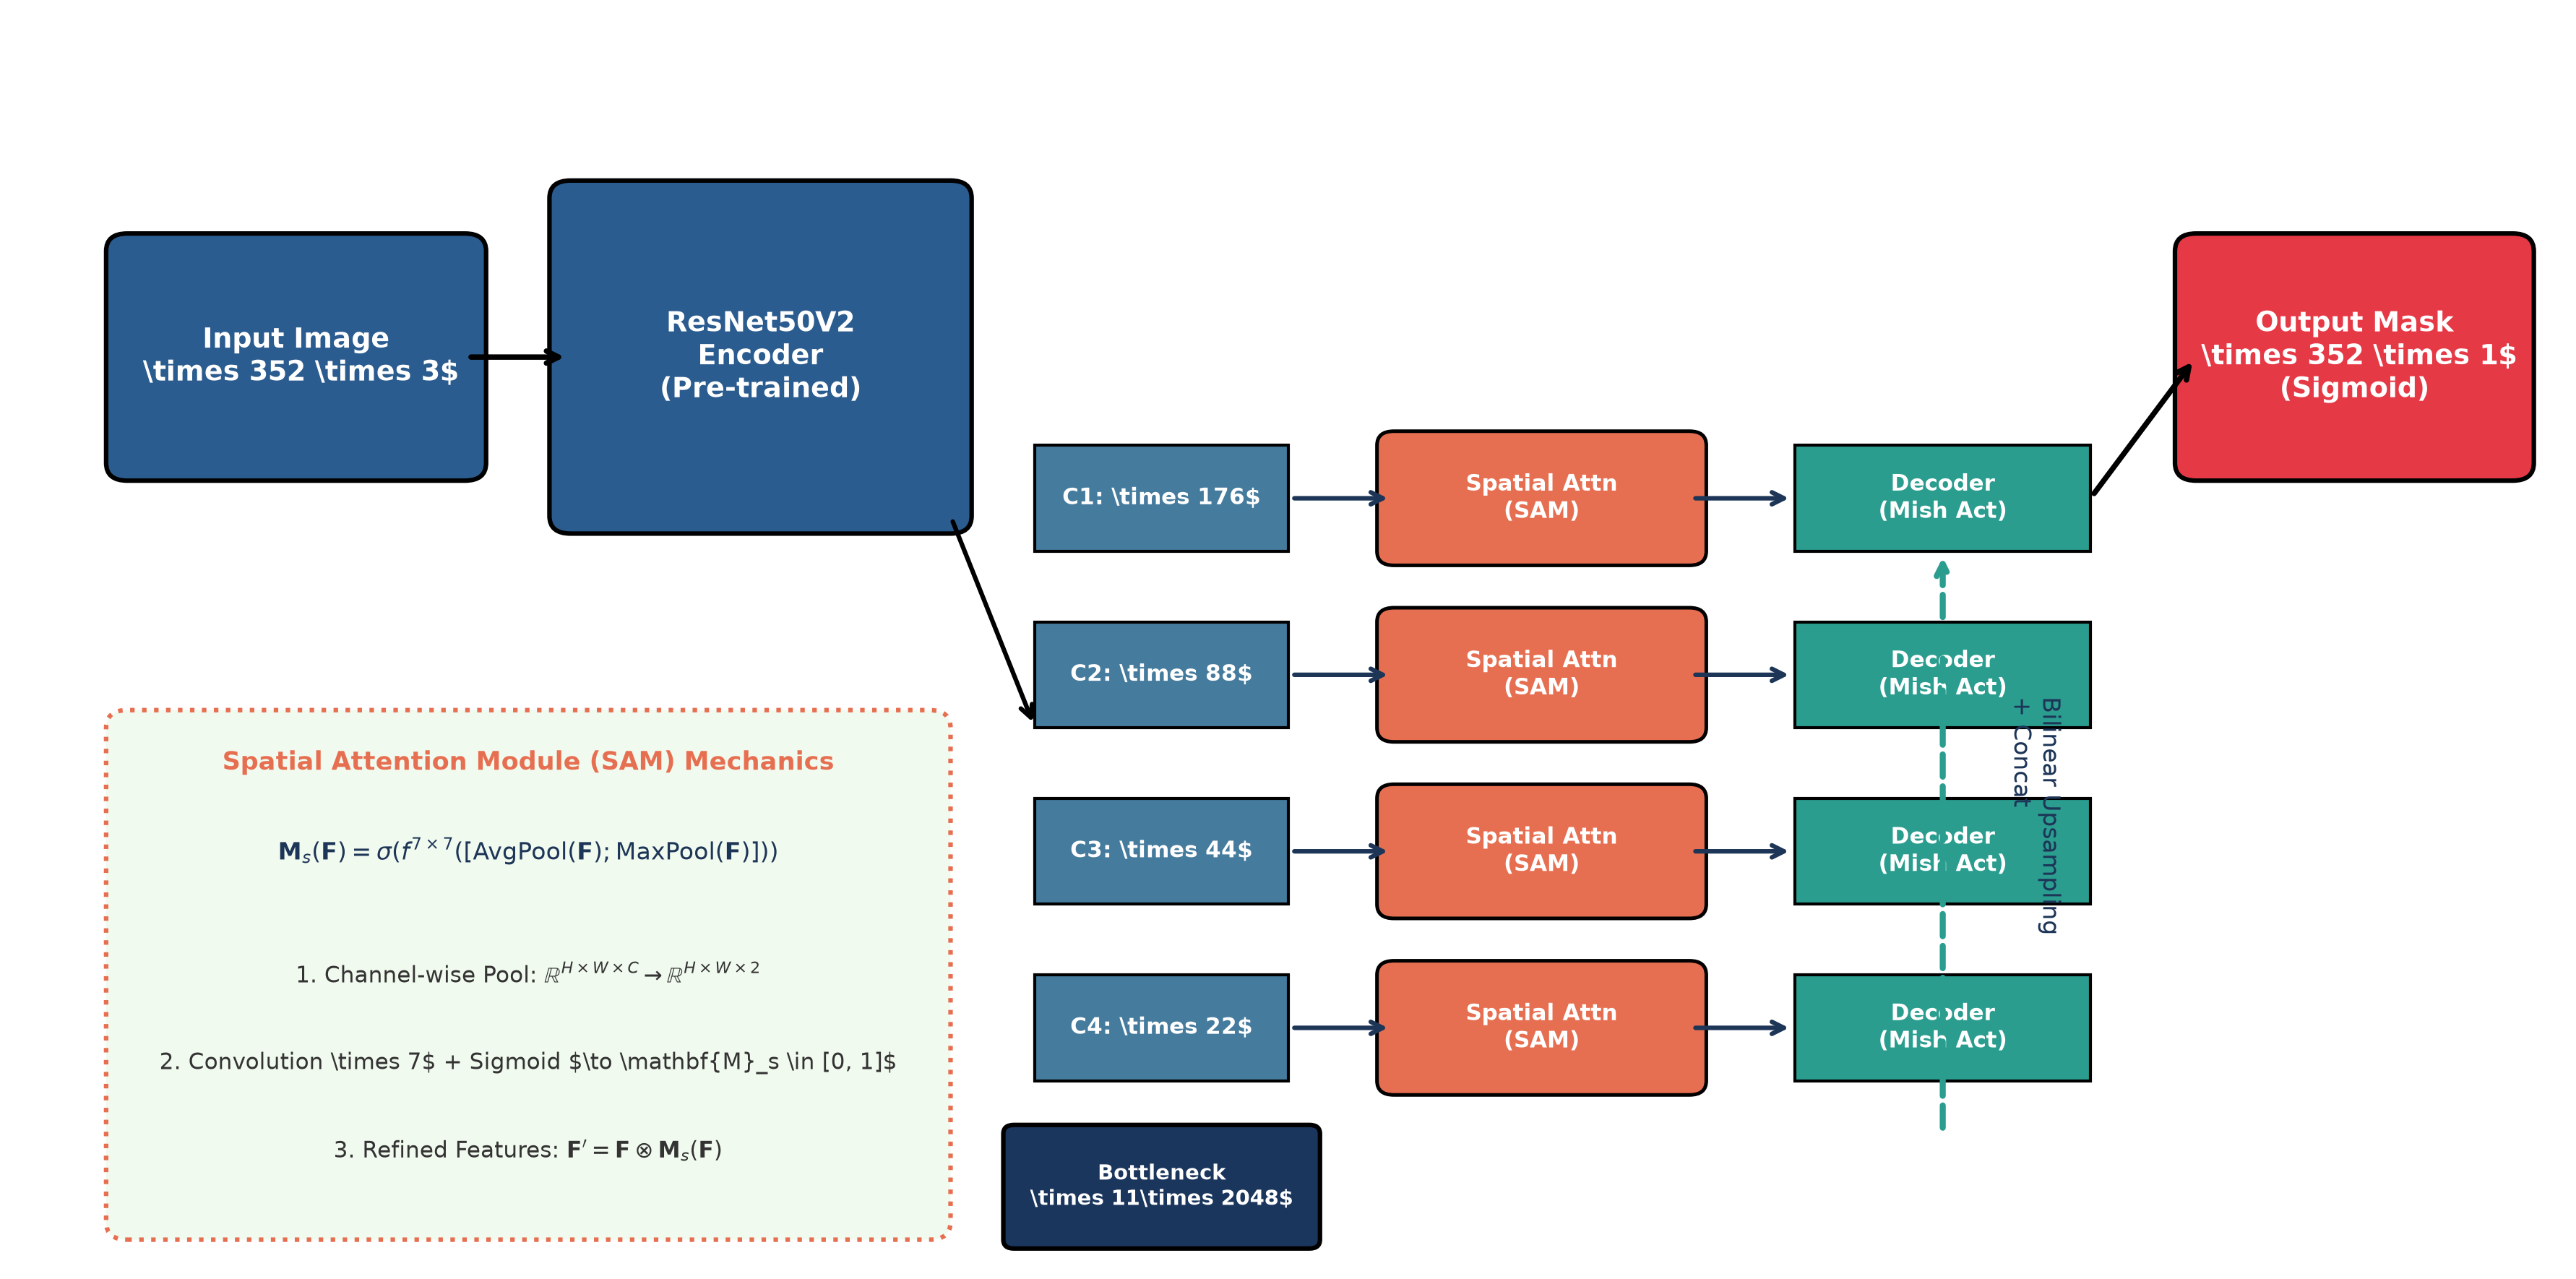
\includegraphics[width=0.98\textwidth]{figures/architecture_rapunet.png}
    \caption{Arquitetura detalhada da rede RAPUNet-Zeta. O codificador ResNet50V2 extrai mapas de caracter\'{i}sticas em 4 n\'{i}veis hier\'{a}rquicos ($C_1$ a $C_4$). As pontes residuais passam pelo M\'{o}dulo de Aten\c{c}\~{a}o Espacial (SAM), sendo em seguida concatenadas com as ativa\c{c}\~{o}es ascendentes processadas por blocos com fun\c{c}\~{a}o Mish.}
    \label{fig:architecture}
\end{figure}

\subsubsection{Codificador Profundo (ResNet50V2 Backbone):}
Ao inv\'{e}s de convolu\c{c}\~{o}es bidimensionais aleatoriamente inicializadas, adota-se o extrator de caracter\'{i}sticas ResNet50V2 \cite{he2016identity} pr\'{e}-treinado sobre o \textit{ImageNet}. As conex\~{o}es de identidade aprimoradas da vers\~{a}o V2 realizam a pr\'{e}-ativa\c{c}\~{a}o antes da convolu\c{c}\~{a}o, facilitando a propaga\c{c}\~{a}o desimpedida dos gradientes durante a etapa de \textit{backpropagation}. Os tensores de caracter\'{i}sticas intermedi\'{a}rios s\~{a}o interceptados em quatro est\'{a}gios de resolu\c{c}\~{a}o espacial decrescente:
$C_1 \in \mathbb{R}^{176 \times 176 \times 64}$, $C_2 \in \mathbb{R}^{88 \times 88 \times 256}$, $C_3 \in \mathbb{R}^{44 \times 44 \times 512}$ e $C_4 \in \mathbb{R}^{22 \times 22 \times 1024}$, culminando no gargalo (\textit{bottleneck}) de $11 \times 11 \times 2048$.

\subsubsection{M\'{o}dulo de Aten\c{c}\~{a}o Espacial (Spatial Attention Module -- SAM):}
Para reproduzir o mecanismo seletivo de aten\c{c}\~{a}o preconizado por trabalhos recentes como LACFormer \cite{lacformer2023}, foi incorporado um operador de aten\c{c}\~{a}o espacial nas \textit{skip connections}. Seja $\mathbf{F} \in \mathbb{R}^{H \times W \times C}$ o mapa de caracter\'{i}sticas oriundo do codificador. O SAM primeiro realiza opera\c{c}\~{o}es de agrupamento espacial m\'{e}dio (\textit{Average Pooling}) e m\'{a}ximo (\textit{Max Pooling}) ao longo do eixo de canais $C$, gerando dois mapas bidimensionais que sintetizam a energia espacial das ativa\c{c}\~{o}es:
\begin{equation}
    \mathbf{F}_{\text{avg}} = \frac{1}{C}\sum_{c=1}^{C} \mathbf{F}_{:,:,c}, \quad \mathbf{F}_{\text{max}} = \max_{c \in \{1,\dots,C\}} \mathbf{F}_{:,:,c}
\end{equation}
Ambos os descritores s\~{a}o concatenados ao longo da dimens\~{a}o de canal e submetidos a uma convolu\c{c}\~{a}o com kernel largo de tamanho $7 \times 7$, seguida pela fun\c{c}\~{a}o de ativa\c{c}\~{a}o sigm\'{o}ide $\sigma(\cdot)$ para calibrar uma m\'{a}scara de pesos normalizada $\mathbf{M}_s \in [0, 1]^{H \times W \times 1}$:
\begin{equation}
    \mathbf{M}_s(\mathbf{F}) = \sigma \left( f^{7 \times 7} \left( [ \mathbf{F}_{\text{avg}} \, ; \, \mathbf{F}_{\text{max}} ] \right) \right)
\end{equation}
O mapa de caracter\'{i}sticas refinado $\mathbf{F}'$ que alimenta o decodificador \'{e} obtido pela multiplica\c{c}\~{a}o elemento a elemento (\textit{Hadamard product}) entre o tensor original e a m\'{a}scara de aten\c{c}\~{a}o espacial:
\begin{equation}
    \mathbf{F}' = \mathbf{F} \otimes \mathbf{M}_s(\mathbf{F})
\end{equation}
Essa formula\c{c}\~{a}o força os coeficientes de regi\~{o}es homog\^{e}neas de fundo escuro a tenderem a zero, amplificando as bordas e gradientes de textura an\^{o}malos caracter\'{i}sticos dos p\'{o}lipos.

\subsubsection{Decodificador com Ativa\c{c}\~{a}o Mish:}
No caminho de expans\~{a}o (decodificador), camadas convolucionais com transposi\c{c}\~{a}o (\textit{UpSampling2D} bilinear) restauram a resolu\c{c}\~{a}o original. Todas as camadas intermedi\'{a}rias de decodifica\c{c}\~{a}o substituem a tradicional fun\c{c}\~{a}o ReLU pela ativa\c{c}\~{a}o suave e n\~{a}o monot\^{o}nica \textit{Mish} \cite{misra2019mish}:
\begin{equation}
    f_{\text{Mish}}(x) = x \cdot \tanh(\text{softplus}(x)) = x \cdot \tanh(\ln(1 + e^x))
\end{equation}
A curvatura suave e a derivada n\~{a}o-nula em regi\~{o}es negativas eliminam a desativa\c{c}\~{a}o permanente de neur\^{o}nios, assegurando estabilidade num\'{e}rica e fluxo ininterrupto de informa\c{c}\~{a}o nos gradientes. A camada final projeta a densidade de probabilidades com ativa\c{c}\~{a}o sigm\'{o}ide em resolu\c{c}\~{a}o $352 \times 352 \times 1$.

\subsection{Fun\c{c}\~{a}o de Custo (Dice Loss)}
Para contrabalan\c{c}ar a severa assimetria de classes cl\'{i}nica --- onde o n\'{u}mero de pixels pertencentes \{a} mucosa saud\'{a}vel supera massivamente os pixels da les\~{o}o --- a rede foi otimizada utilizando diretamente a \textit{Dice Loss}, derivada do \textit{Dice Similarity Coefficient} (DSC):
\begin{equation}
    \mathcal{L}_{\text{Dice}}(Y, \hat{Y}) = 1 - \frac{2 \sum_{i=1}^{N} y_i \hat{y}_i + \epsilon}{\sum_{i=1}^{N} y_i + \sum_{i=1}^{N} \hat{y}_i + \epsilon}
\end{equation}
onde $y_i \in \{0, 1\}$ denota o r\'{o}tulo verdadeiro do $i$-\'{e}simo pixel, $\hat{y}_i \in [0, 1]$ representa a probabilidade predita pelo modelo, e $\epsilon = 10^{-5}$ \'{e} um termo de suaviza\c{c}\~{a}o para evitar divis\~{o}es por zero.
